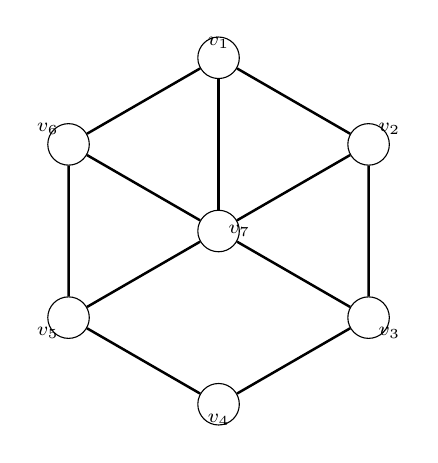
\begin{tikzpicture}[
  scale=1.0,
  vertex/.style={circle, draw=black, fill=white, inner sep=0pt, minimum size=15pt},
  every node/.style={font=\small}
]
  \node[vertex] (v1) at (90:2.2) {};
  \node[vertex] (v2) at (30:2.2) {};
  \node[vertex] (v3) at (-30:2.2) {};
  \node[vertex] (v4) at (-90:2.2) {};
  \node[vertex] (v5) at (-150:2.2) {};
  \node[vertex] (v6) at (150:2.2) {};
  \node[vertex] (v7) at (0,0) {};

  \draw[line width=0.9pt] (v1) -- (v2) -- (v3) -- (v4) -- (v5) -- (v6) -- (v1);
  \draw[line width=0.9pt] (v7) -- (v1);
  \draw[line width=0.9pt] (v7) -- (v3);
  \draw[line width=0.9pt] (v7) -- (v5);
  \draw[line width=0.9pt] (v2) -- (v7);
  \draw[line width=0.9pt] (v6) -- (v7);

  \node[font=\scriptsize, above] at (v1) {\(v_1\)};
  \node[font=\scriptsize, above right] at (v2) {\(v_2\)};
  \node[font=\scriptsize, below right] at (v3) {\(v_3\)};
  \node[font=\scriptsize, below] at (v4) {\(v_4\)};
  \node[font=\scriptsize, below left] at (v5) {\(v_5\)};
  \node[font=\scriptsize, above left] at (v6) {\(v_6\)};
  \node[font=\scriptsize, right] at (v7) {\(v_7\)};
\end{tikzpicture}
